\IEEEPARstart{V}ision-to-Language problems present a particular challenge in Computer Vision because they require translation between two different forms of information.  In this sense the problem is similar to that of machine translation between languages. In machine language translation there have been a series of results showing that good performance can be achieved without developing a higher-level model of the state of the world. In~\cite{bahdanau2014neural,cho2014learning,sutskever2014sequence}, for instance, a source sentence is transformed into a fixed-length vector representation by an `encoder' RNN, which in turn is used as the initial hidden state of a `decoder' RNN that generates the target sentence.

Despite the supposed equivalence between an image and  a thousand words, the
manner in which information is represented in each data form could hardly be
more different. Human language is designed specifically so as to communicate
information between humans, whereas even the most carefully composed image is
the culmination of a complex set of physical processes over which humans have
little control.  Given the differences between these two forms of information,
it seems surprising that methods inspired by machine language translation have
been so successful. These RNN-based methods which translate directly from image
features to text, without developing a high-level model of the state of the
world, represent the current state of the art for key Vision-to-Language (\V2L)
problems, such as image captioning and visual question answering.

This approach is reflected in many recent successful works on image captioning, such as~\cite{Chen2015CVPRMind,donahue2014long,karpathy2014deep,mao2014deep,vinyals2014show,yao2015describing,devlin2015language}.
Current state-of-the-art captioning methods use a CNN as an image `encoder' to produce a fixed-length vector representation~\cite{krizhevsky2012imagenet,lecun1998gradient,simonyan2014very,szegedy2014going}, which is then fed into the `decoder' RNN to generate a caption.

\begin{figure}[t!]
\centering
  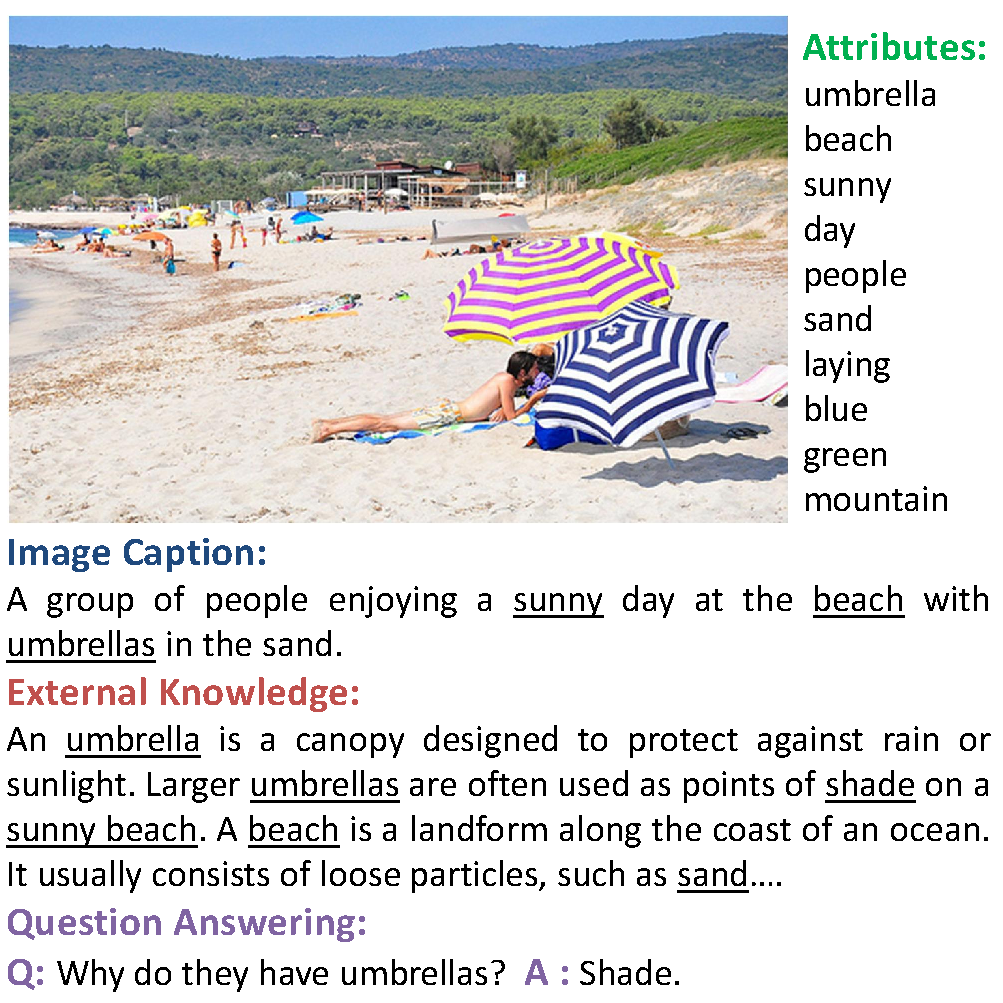
\includegraphics[width=0.9\linewidth]{./img/titile_example_fig_real.pdf}
  \vspace{-5pt}
  \caption{
    An example of the proposed \V2L system in action. Attributes are predicted by our CNN-based attribute prediction model.
    Image captions are generated by our attribute-based captioning generation model.
    %
    %
    All of the predicted attributes and generated captions, combined with the mined external knowledge
    from a large-scale knowledge base, are fed to an LSTM to produce the answer to the asked question.
    Underlined words indicate the information required to answer the question.}
  \label{img:example}
  \vspace{-15pt}
\end{figure}


Visual Question Answering (VQA) is a more recent challenge than image captioning. It is distinct from many problems in Computer Vision because the question to be answered is not determined until run time~\cite{antol2015vqa}. %
In this \V2L problem an image and a free-form, open-ended question about the image are presented to the method which is required to produce a suitable answer~\cite{antol2015vqa}. As in image captioning,
 the current state of the art in VQA~\cite{gao2015you,malinowski2015ask,ren2015image}
 relies on passing CNN features to an RNN language model.
 However, visual question answering is a significantly more complex problem than image captioning, not least because it requires accessing information not present in the image.  This may be common sense, or specific knowledge about the image subject. For example, given an image, such as Figure \ref{img:example}, showing `a group of people enjoying a sunny day at the beach with umbrellas', if one asks a question `why do they have umbrellas?', to answer this question, the machine must not only detect the scene `beach', but must know that `umbrellas are often used as points of shade on a sunny beach'. Recently, Antol \etal~\cite{antol2015vqa} also have suggested that VQA is a more ``AI-complete'' task since it requires multimodal knowledge beyond a single sub-domain. %

The contributions of this paper are two-fold.
First, we propose a {\em fully trainable} attribute-based neural network founded upon the CNN+RNN architecture,
that can be applied to multiple \textit{V2L} problems.
We do this by inserting an explicit representation of attributes of the scene which are meaningful to humans.
Each semantic attribute corresponds to a word mined from the training image descriptions, and represents higher-level
knowledge about the content of the image. A CNN-based classifier is trained for each attribute,
and the set of attribute likelihoods for an image form a high-level representation of image content.
An RNN is then trained to generate captions, or question answers, on the basis of the likelihoods.
Our attribute-based model yields significantly better performance than current state-of-the-art approaches in the task of image captioning. %

Based on the proposed attribute-based \textit{\V2L} model,
%
%
our second contribution is to introduce 
%
a method of incorporating knowledge external to the image, including common sense, into the VQA process.
%
In this work, we fuse the automatically generated description of an image with information extracted from an external
knowledge base (KB) to provide an answer to a general question about the image (See Figure \ref{frame}). The image description takes the form of a set of captions, and the external knowledge is text-based information mined from a Knowledge Base. Specifically, for each of the top-$k$ attributes detected in the image we generate a query which may be applied to a Resource Description Framework (RDF) KB, such as DBpedia.  RDF is the standard format for large KBs, of which there are many.  The queries are specified using Semantic Protocol And RDF Query Language (SPARQL). We encode the paragraphs extracted from the KB using Doc2Vec \cite{le2014distributed}, which maps paragraphs into a fixed-length feature representation. The encoded attributes, captions, and KB information are then input to an LSTM which is trained so as to maximise the likelihood of the ground truth answers in a training set. We further propose a question-guided knowledge selection scheme to improve the quality of  the extracted KB information. The knowledge that is
not related to the question is filtered out. The approach that we propose here combines the generality of information that using a KB allows with the generality of questions that the LSTM allows.
In addition, it achieves an accuracy of 70.98\% on the Toronto COCO-QA~\cite{ren2015image}, while the latest state of the art is 61.60\%. On the VQA~\cite{antol2015vqa} evaluation server (which does not publish ground truth answers for its test set), we also produce the state-of-the-art result, which is 59.50\%.

A preliminary version of this work was published at CVPR 2016 \cite{wu2015image,wu2015ask}. The new material in this paper comprises further experiments on two additional VQA datasets. More ablation models of the original model are implemented and studied. More importantly, a new model (A+C+Selected-K-LSTM) 
%
is introduced 
%
for the visual question answering task, leading to a new state-of-the-art result.




